\section{Methodology}\label{Methodology}

\subsection{Feedback fuzzing as Markov Decision Process}

\begin{figure}[t]
	\centering
	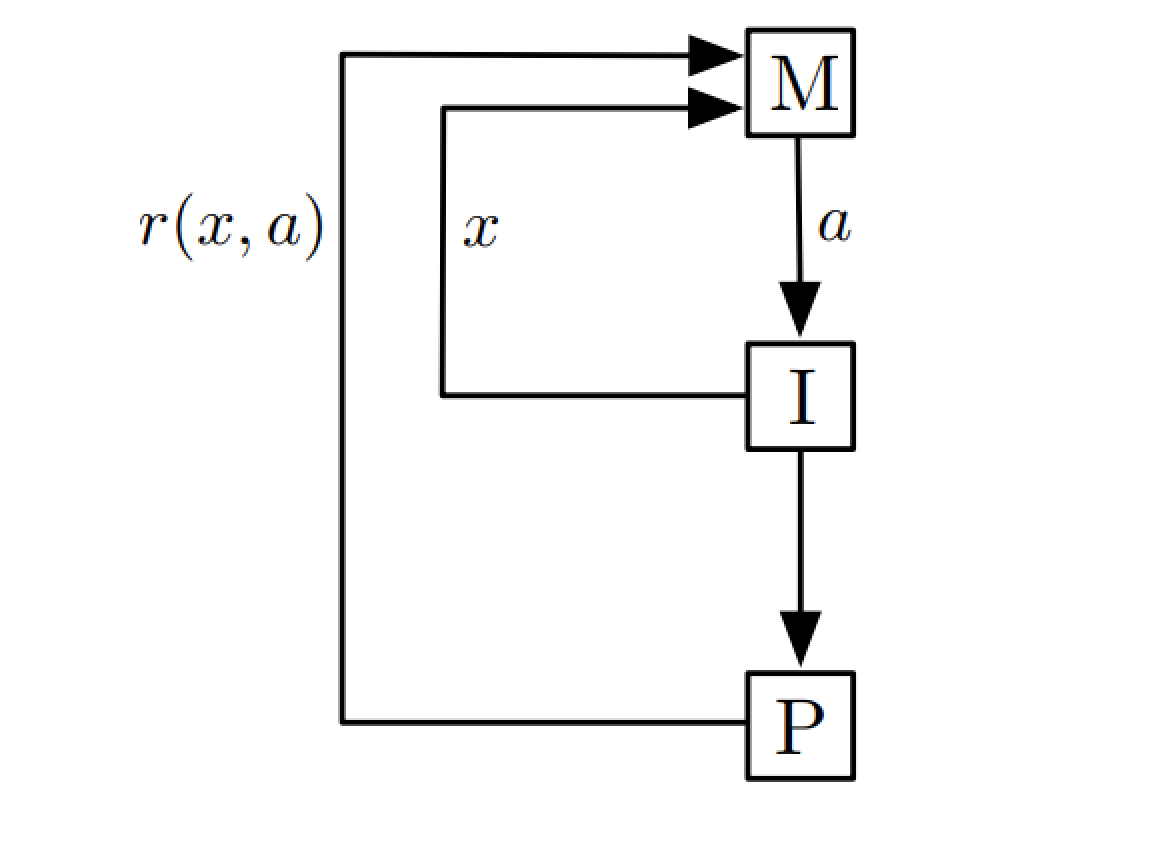
\includegraphics[width=2in]{pic/modeling.png}
	\caption{Feedback fuzzing as Markov Decision process}
	\label{modeling}
\end{figure}

Feedback based fuzzing can be modeled as learning process with a feedback loop. Initially, the fuzzer generates new inputs, and then runs the target program with each of them. For each program execution, the fuzzer extracts runtime information (gathered for example by binary instrumentation) for evaluating the quality (with respect to the defined search heuristic) of the current input. For instance, this quality can be measured as the number of (unique or not) instructions executed, or the overall runtime of the execution. By taking this quality feedback into account, a feedback-driven fuzzer can learn from past experiments, and then generate other new inputs hopefully of better quality. This process repeats until a specific goal is reached, or bugs are found in the program. Similarly, the reinforcement learning setting defines an agent that interacts with a system. Each performed action causes a state transition of the system. Upon each performed action the agent observes the next state and receives a reward. The goal of the agent is to maximize the total reward over time.

An input mutator engine M generates a new input I by performing a fuzzing action a, and subsequently observes a new state x directly derived from I as well as a reward r(x,a) that is measured by executing the target program P with input I.

More specificlly, we using formaluate the feedback greybox fuzzing as Markov decision process by defining states, action, and reward in the fuzzing context.

\subsubsection{States}
We consider the system that the agent learns to interact with to be a given "seed" projram input. Further, we define the states that the agent observes to be substrings of consecutive symbols within such an input. Formally, let $\sum$ denote a finite set of symbols. The set of possible program inputs $I$ written in this alphabet is then defined by the Kleene closure $I : = \sum^{*}$. For an input string $x = x_{1}, ..., x_{2} \in I$, let
$$S(x) := {(x_{1+i}, ..., x{m+i} | i\geq 0, m+n \leq n)}$$
denote the set of all substrings of x. Clearly, $\cup_{x\in I}S(x) = I$ holds. We define the states of out Markov decision process to be $I$. In the following, $x\in I$ denotes an input for the target program and $x^{'} \in S(x) \subset I$ a substring of this input..

\subsubsection{Actions}
We define the set of possible actions $A$ of our Markov decision process to be random variables mapping substrings of an input to probabilistic rewriting/ mutation rules:

$$A:={a:I \rightarrow (I \times I, F, P)|a~\pi(x^{'})}$$

where $F = \sigma (I \times I)$ denotes the $\sigma$-algebra of the sample space $(I \times I)$ and P gives the probability for a given rewrite rule. In our Implementation, we define a small subset $A \subset A$ probabilistic string rewrite rules that operate on a given seed input.

\subsubsection{Rewards}
We define rewards independently for both characteristics of (1): the next preformed action $a$ and (2) the program execution with the next generated input x, i.e. $r(x,a)$= $E(x)$+$G(a)$.
In our implementation, we experiment with E providing the numbers of newly discoverd bsic blocks, execution path length,  and execution time of the target that processes the input x. For example, we can define the number of newly discovered blocks as 
$$E_{1}(x, I^{'} := |B(c_{x} \setminus) (\cup_{x\in I^{'}}B(c_{x}))|)$$
where $c_{x}$ denotes the execution path the target program takes when processing input x, $B(c_{x})$ is the set of unique basic blocks of this path, and $I^{'} \subset I$ is the set of previously processed inputs. Here, we define a basic block as a sequence of program instructions without branch instructions.

\subsection{Guided feedback fuzzing as Reward optimization problem}

Now we modeling the feedback greybox fuzzing as the Markov decision process. Furthermore, the  guided feedback greybox fuzzing could be cast into objected optimization problem. The object is to maximize the feedback reward.

The official AFL exploit the qualitative reward feedback, i.e. if the test case trigger new block to block transition) to saving interesting test case and mutate it to achieve the goal of coverage more new branch. AflFast use the quantitative reward(branch hit number) as reward to mutate more test case based on test case that trigger low frequency path, its goal is also to maximize the code coverage more efficiency.

Beside the goal of maximize the coverage,  we could achieve other optimization object by choosing highly-rewarded actions and spending more resource on the highly-reward actions.

For example, if the feedback reward is the quantitative depth of execution path. Based on our institution that the deeper we explore, the more change we could find vulnerabilities. Our guided fuzzing goal maybe to reach the deepest path as soon as possible, then we could choose and spend more resource on those test case that explore deeper.

If the feedback reward is the quantitative complex degree of execution path, and based on institution that the more complex area, the more chance to be vulnerable. Our goal of guided fuzzing maybe to explore the most complex path as soon as possible, then we could choose and spend more resource on these test cast that explore more complex path.

If the feedback reward is the connection degree from its neighborhood of the execution path, and based on our institution that if the connection degree is lesser, the fair reach of these area, and the fairer to reach, the more chance to have bugs in these fair reach areas. Our goal of guided fuzzing maybe to execute the most fair reach areas as soon as we can. Then we could choose and spend more resource on these test case that explore  fairer reach areas.

So far, we  cast the goal guided feedback fuzzing as the object optimization problem to achieving the highest reward as soon as possible.

\subsection{Fish School Search based Energy Scheduler}

Now we have the goal like exploring the deepest path, the most complex path, the fairest reach path as soon as possible. And we know where to spend more resource according to the different goals. If our goal is to execute the deepest, we will chose the test case that executed deeper path, and spend more resource on the test case (specify we mutate more test case based on the test case.)

Then we know we should spend more resource on these test case that its reward is higher, and the higher the reward, the more resource we should spend. But how much more resource is spent is another balance problem.

We borrow the ideas of movement operators from fish school search algorithm. The core idea is to make the fishes “swim” toward the positive gradient in order to “eat” and “gain weight”. Collectively, the heavier fishes are more influent in the search process as a whole, what makes the barycenter of the fish school moves toward better places in the search space over the iterations.

Similarly, we model the execution of one test case as swim of one fish,  and reward it obtain along the path is regarded as "weight", the heavier test case will have more in influence and attract more resource. Then other fishes(test cases) will follow the heavier fish. We modeling the resource distribution as the movement operators of fish school search algorithm.


We design three strategies of quantitative resource distribution : constant, linear, exponential and sqrt.

If the total reward of each execution of one test case is donated as $TotalReward(T) = \sum Reward(BB_{i})$ where, $BB \in Path(T)$. We update the Maximize path weight,  Minimize path weight, and calculate the average path weight (i.e. $AvgPathWeight= MaximinzePath + MinimizePath /2$) as the \textbf{KEY } parameter for energy assignment.



